\documentclass{article}[12pt]

% GRAPHICS
\usepackage{float}
\usepackage{graphicx}
\usepackage{subcaption}

% HYPERLINKS
\usepackage{hyperref}

% DOCUMENT PADDING AND MARGINS
\usepackage{titlesec}
\usepackage[margin=1.0in]{geometry}
\setlength{\parskip}{\baselineskip}%
\setlength{\parindent}{0pt}
\titlespacing*{\section}{0pt}{2ex}{0ex}
\titlespacing*{\subsection}{0pt}{1ex}{-2ex}
\titlespacing*{\subsubsection}{0pt}{2ex}{-2ex}

%COMMENTING
\usepackage{comment}
\begin{document}

% TITLE
\vspace{-5cm}
\title{Autonomous Quadrotor Landing on a Moving Platform}
\author{Stan Brown \& Chris Choi}
\date{}
\maketitle

\section*{Introduction}
The goal of this project is to develop a set of controllers and methods that allow a quadcopter equipped with a downward facing camera and sonar to perform fully autonomous landing on a moving platform without relying on high accuracy GPS measurements. In this interim report we provide an update on the progress made so far on the software and hardware aspects, as well as changes made to the project scope. Additionally we provide an updated project schedule for the remainder of the term. 

\section*{Project Progress}
\subsection*{Hardware Status}
\subsubsection*{Flight Controller and Quadroter}
For the flight controller, which handles the low level control loops and keeps the quadrotor steady, we have selected a Pixhawk v2.4 running the PX4 firmware stack, and for the quadrotor frame we have selected a DJI 450 Flamewheel. The powertrain of the quadrootr consistes of a set of Emax 2213-935KV motors with complimentary 1045R propellers, a Thunder Power lipo 11.1V 4200mah battery, and a set of DJI E310 420S 20A electronic speed 
controllers. At current our quadrotor flies \textit{reasonably well} with some \textit{minor} setbacks, mainly due to the instability of the firmware, and lack of documentation for the firmware 
and software packages. The project setbacks thus far have almost all been entirely related to PX4 firmware stack. Figure \ref{hardware} shows the state of the quadrotor at the time of this report. 

\begin{figure}[]
	\centering
	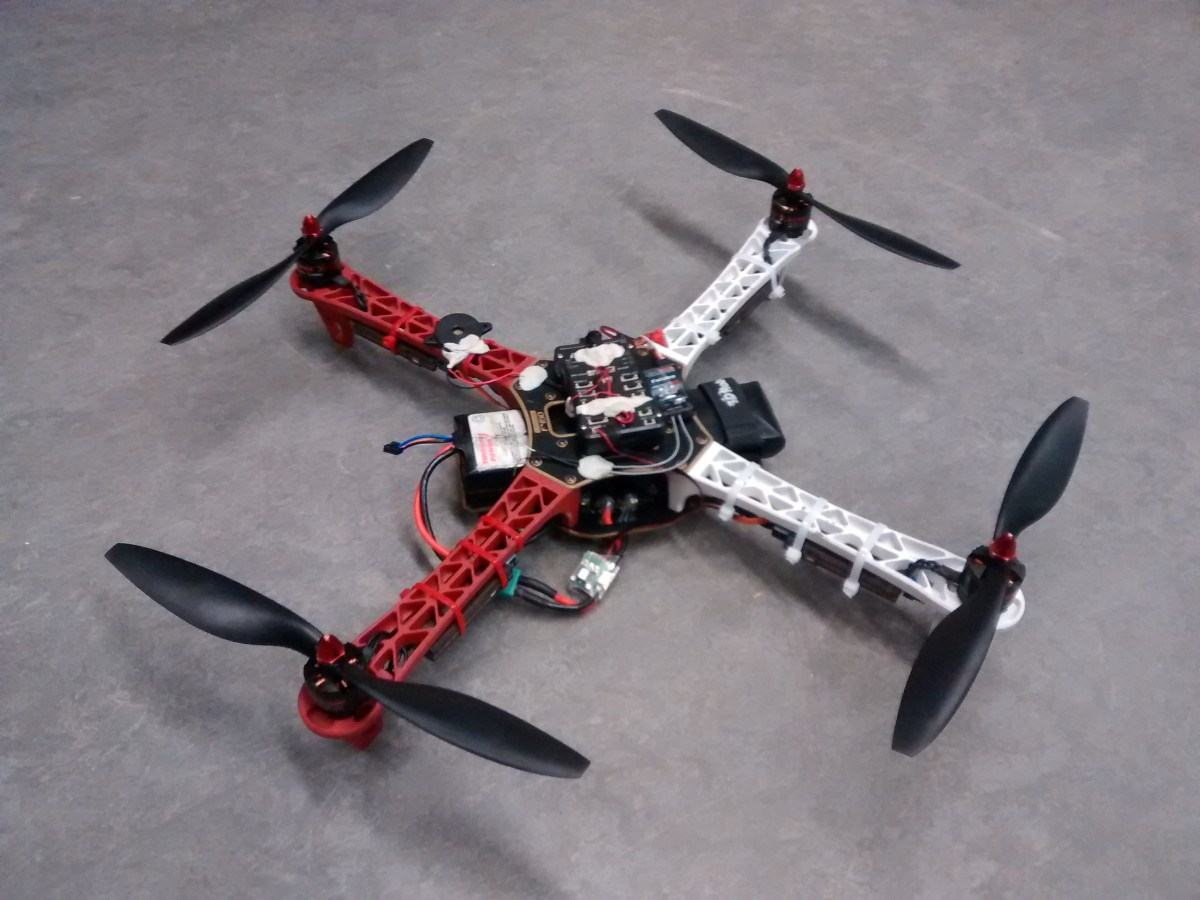
\includegraphics[width=0.6\linewidth]{images/quadrotor.jpg}
	\caption{DJI F450 with Pixhawk v1.5}
	\label{hardware}
\end{figure}

\subsubsection*{Onboard Autonomous Control System and Vision Processing}
For high level control and vision processing we have selected an Odroid XU4 microcomputer because of its small size, low weight, low power consumption relative to its processing power. The Odroid will be mounted on the quadrotor frame and will be powered directly from the quad rotor battery pack. 

Visual data will, for now,  be captured using a Logitech C270 HD webcam whcih runs at a frame rate of 25Hz. We plan to use this web cam for the initial testing stages and once we are confident in the high level control systems such that the chance of an accident occurring as the result of a software glitch is considered low we will upgraded to a Ximia xiQ USB3 camera. Compared to the Logitech web cameara, the Ximia camera has a number of additional features, such as a higher frame rate (60Hz), interchangeable lenses and a set ROS drivers that can access the `al camera settings.


\subsection*{Software}
\subsubsection*{Pixhawk Firmware}
As mentioned in the hardware section, we have had numerous issues using the software suite for the Pixhawk Flight Controller, as well as the PX4 firmware itself. There are many instances where we could not explain the instability of the quadrotor during flight, many of which lead to 
costly crashes, but we believe through these experiences we have developed a 
procedure to lower the risk for such instances from happening often.

\subsubsection*{Odriod to Pixhawk Communication}
For our autonomous system to control the quadrotor directly, the Odriod has to 
be able to communicate with the Pixhawk, this is where \verb|mavros| (ROS 
package) comes into play. Mavlink is a popular UAV communication protocol 
between UAV and ground control softwares, \verb|mavros| creates a mavlink ROS 
node to enable developers to monitor and issue mavlink commands with ease. We 
have successfully used mavros to arm and disarm Pixhawk (tested), in the near 
future we should be able to send velocity/attitude commands to control the 
quadrotor.

\subsubsection*{Simulator}
Initially we explored the possibility of using the combination of PX4's 
Software in the Loop Simulation (SITL) and Gazebo 6 as our simulation 
environment for our project, however we found the combination of poor installation instructions that were inconsistently updated along with poor, often outdated, documentation major concern for us. After spending more than 15 hours in attempting to install and run the simulator we have decided to abandon the SITL simulation and create a simple simulation in Matlab to test our estimation and control loops. We therefore implicitly assume that the Pixhawk will execute any velocity/attitude commands accurately and without any delays. 

\subsubsection*{AprilTag Software}
Using a set of April tags and camera calibration functions provided in the OpenCV library, we been able to successfully obtained accurate pose estimations between the Logitech webcam and a single AprilTag. The translational error in the pose estimation appears to be below $\pm 1$ cm while the rotational error has not yet been measured. We plan to use the Optitrack Motion capture system system currently installed in the lab to take a large set of measurements in order to provide an accurate estimation of the errors associated with using the AprilTag Software. 

The current rate AprilTag software operates at 20 fps on the Odroid and we will investigate a modified version of the AprilTag library made by Kevin Ling, a former Wave Lab member who optimitize the AprilTag source code in a previous project. We have also successfully measured the pose from two April tags simultaneously by placing a small AprilTag inside a larger one such that when the larger AprilTag goes out of the cameras FOV measurements pose estimates will be provided by the smaller one. This has the advantage of continuously providing pose estimation with the quadrotor is less than a meter above the target which is point at which a 40cm by 40cm april tag goes out of the camera view. An example of the two AprilTags providing simultaneous measurements is shown in Figure \ref{fig:apriltag}.

\begin{figure}[]
	\centering
	\begin{subfigure}[b]{0.45\linewidth}
		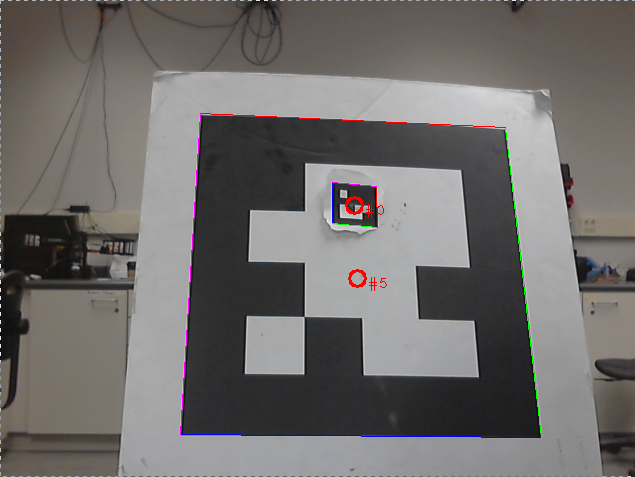
\includegraphics[width=\textwidth]{images/apriltags_1.png}
		\caption{2 Apriltags Detected}
	\end{subfigure}
	\begin{subfigure}[b]{0.45\linewidth}
		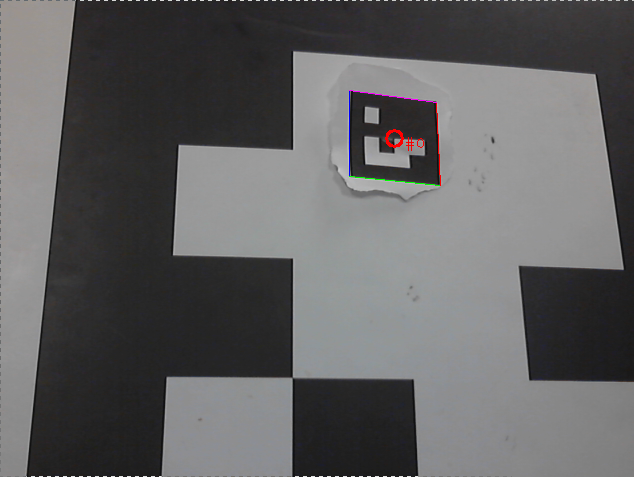
\includegraphics[width=\textwidth]{images/apriltags_3.png}
		\caption{1 Apriltag Detected }
	\end{subfigure}
	\caption{Apriltag Inception - By using secondary AprilTag inside a larger one the FOV problem associated with AprilTags when the camera is either to far away or two close is avoided.}
	\label{fig:apriltag}
\end{figure}

\section*{Alterations to Project Scope}
Due to unforeseen difficulties in getting the software and hardware to interface with each other along with difficulties in getting an accurate simulation operational we will no longer be using a gimballed camera for this stage of the project. We had initially hoped to use attach gimbal to the downward facing camera on the quadcopter to make tracking the target easier in cases where the quadrotor is required to make rapid corrections.

The removal of the gimbal only pertains to the portion of the project that will be completed by the end of this academic term (April 2016) and we plan to revisit once we have a base solution that works in situations where there is low wind and the platform is moving relatively slowly. A new updated project schedule is summarized in the next section.

\section*{Schedule}

\begin{itemize}
	\vspace{-0.2cm}
	\setlength{\itemsep}{5pt}
	\setlength{\parskip}{0pt}
	\setlength{\parsep}{0pt}
	
	\item{\textbf{6th March}: Implement and show in simulation that we can land 
	a quadrotor successfully on to a moving platform}
	\item{\textbf{21st March}: Perform autonomous flying indoors}
	\item{\textbf{13th March}: Perform autonomous flying outdoors}
	\item{\textbf{28th March}: Attempt to autonomous land the quadrotor Indoors}
\end{itemize}






\bibliography{proposal}{}
\bibliographystyle{ieeetr}

\end{document}
